% !TEX root = catron-dissertation.tex
\epstopdfsetup{outdir=./images/06_single_sensor_filtering/}

\chapter{Wavefront Multidimensional Spectral Filtering Techniques}
\label{chap:06_single_filter}
% \textcolor{red}{
%   \begin{itemize}
%     \item Work on the chapter intro
%     \item Filter applied in Fourier space and multidimensional spectral space
%   \end{itemize}
% }

This chapter will examine a variety of filtering techniques used on multidimensional spectra of optical wavefronts.
While none of the filters presented here are novel, many are based on well known digital filters, their application to filtering optical wavefronts is something that needs to be studied.
This chapter will start out by examining some filters that are applied to just the wavefront data itself and will then examine a filtering technique that incorporates additional sensors data in the filtering process.

By using multidimensional spectral estimates on wavefronts, as shown in Chapter \ref{chap:04_dispersion}, differences in source disturbances become clearly evident.
When just the wavefront measurement itself is available, digital filters can be used to separate or isolate a single disturbance source or at least minimize the impact from other sources.
The digital filters used in this dissertation, use a transfer function, $H(j\omega)$, and are applied in Fourier space.
The transfer functions themselves are typically derived in Laplace space, $H(s)$, but because $s=j\omega$ they are valid in Fourier space as well \cite{Hamming-1998-CdhcDuvZ}.
The transfer function is composed of two components which attenuate the signal, gain and phase.
The filter gain is the magnitude of the transfer function, $G(\omega) = |H(j\omega)|$, while the filter phase is the argument, $\Phi(\omega) = \arg(H(j\omega))$.
In the simplest case, the filtered signal is the inverse Fourier transform of the gain multiplied by the Fourier transform of the signal,
\begin{equation}
 f_F(\mathbf{x}) = \real\left(\ifftn[H(j\mathbf{\omega})\fftn\{\mathbf{x}\}]\right) \textrm{,}
 \label{eqn:06_filter_function}
\end{equation}
where $f$ is the signal function and $f_F$ is the filtered signal.

\section{Temporal Filter Methods}
The methods presented in this section are based on Butterworth filters but could be extended to other types of filters.
The square of the transfer function of a Butterworth filter is \cite{Butterworth-1930-DvDrjKha},
\begin{equation}
 |H(j\omega)|^2 = G^2(\omega) = \frac{G_0^2}{1+\left(\frac{j\omega}{j\omega_c}\right)^{\pm2n}} \textrm{,}
 \label{eqn:06_butterworth}
\end{equation}
where $G_0$ is the zero-frequency gain, $\omega_c$ is the cutoff angular frequency, $n$ is the filter order (number of filters in a series), and $\pm$ represents either a low-pass ($+$) or high-pass ($-$) filter.
The gain of this filter is
\begin{equation}
  G(\omega) = \frac{G_0}{\sqrt{1+\left(\frac{\omega}{\omega_c}\right)^{\pm2n}}} \textrm{.}
  \label{eqn:06_butterworth_gain}
\end{equation}
A band-pass filter can be constructed by placing a low-pass filter in series with a high-pass filter and a band-stop by placing the two types in parallel.

In many tests, a large portion of the wavefront noise is at low frequencies primarily caused by mechanical vibration.
In general, a high-pass filter is useful in temporal space for removing this noise, since in many cases most of the power in the aero-optical signal occurs at higher frequency than the low-frequency mechanical vibration. as shown in Figure \ref{fig:06_filter_temporal}.
\begin{figure}
 \centering
 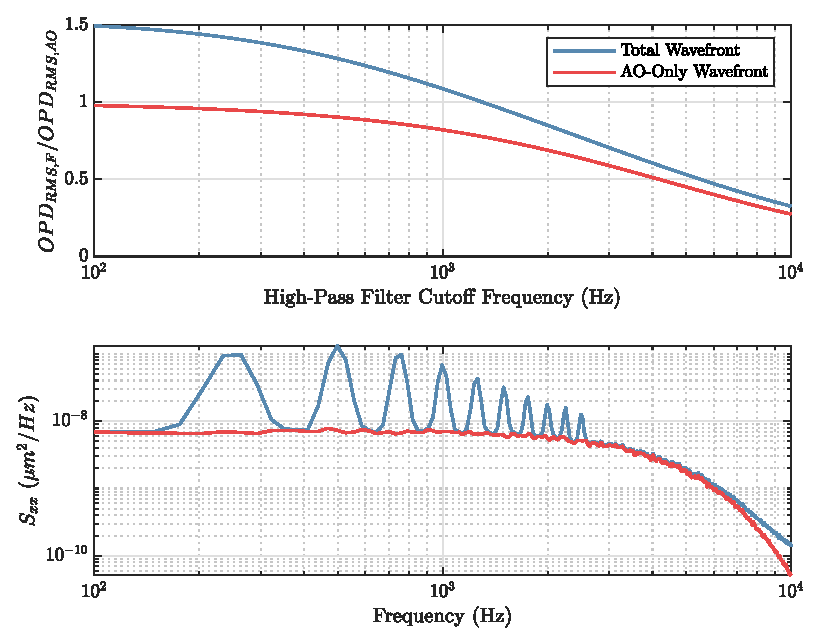
\includegraphics{../matlab/06_single_sensor_filtering/filter_temporal.eps}
 \caption{The $opdrms$ of high-pass temporal filtered wavefronts relative to the $opdrms$ of the aero-optical only unfiltered wavefront (top). Power spectra of both of the simulated wavefront versions (bottom).}
 \label{fig:06_filter_temporal}
\end{figure}
The top plot in this figure shows the high-pass filtered $\opdrms$ of both the total and aero-optical only wavefronts normalized by the unfiltered $\opdrms$ of the aero-optical only wavefront, for high-pass filters with various cutoff frequencies.
The results in Figure \ref{fig:06_filter_temporal} were computed using wavefronts that were simulated using the methods described in Chapter \ref{chap:05_synthetic}.
For reference, the bottom plot of Figure \ref{fig:06_filter_temporal} shows the power spectra of just the aero-optical portion of the wavefront (red curve) and the total wavefront (blue curve) which includes vibration-related peaks associated with the blade-passing frequency and its harmonics.
The figure shows how a high-pass filter decreases the energy in the total wavefront and in the actual aero-optical wavefront, as the filter cutoff frequency increases.
As shown in the top plot, at low cutoff frequency, the filter primarily removes vibration effects from the total signal; however, as the cutoff frequency increases, the filter also removes actual aero-optical signal.
Around 1,200 Hz, the $\opdrms$ of the total signal is equal to the $\opdrms$ of the actual aero-optical signal; at this cutoff frequency ~75\% of the aero-optical signal remains and the remaining signal is made up by the remaining contamination.
This approach can provide a computationally inexpensive way of estimating the aero-optical portion of the wavefront for calculations that rely on the $\opdrms$ of a wavefront.
While it is more straightforward to determine a cutoff frequency for this synthetic wavefront since all of the signal components are fully known, a measured wavefront will likely take some knowledge or expectation of the contamination that is present in the measurement in order to select a high-pass filter cutoff frequency.

% \ref{tab:test}
% \begin{table}
% \centering
% \caption{Test Table}
% \input{../matlab/04_basic_filtering/filter_temporal.txt}
% \label{tab:test}
% \end{table}

An example of wavefronts that result from band-pass and band-stop filtering is shown in Figure \ref{fig:06_filter_temporal_bandpass}.
\begin{figure}
 \centering
 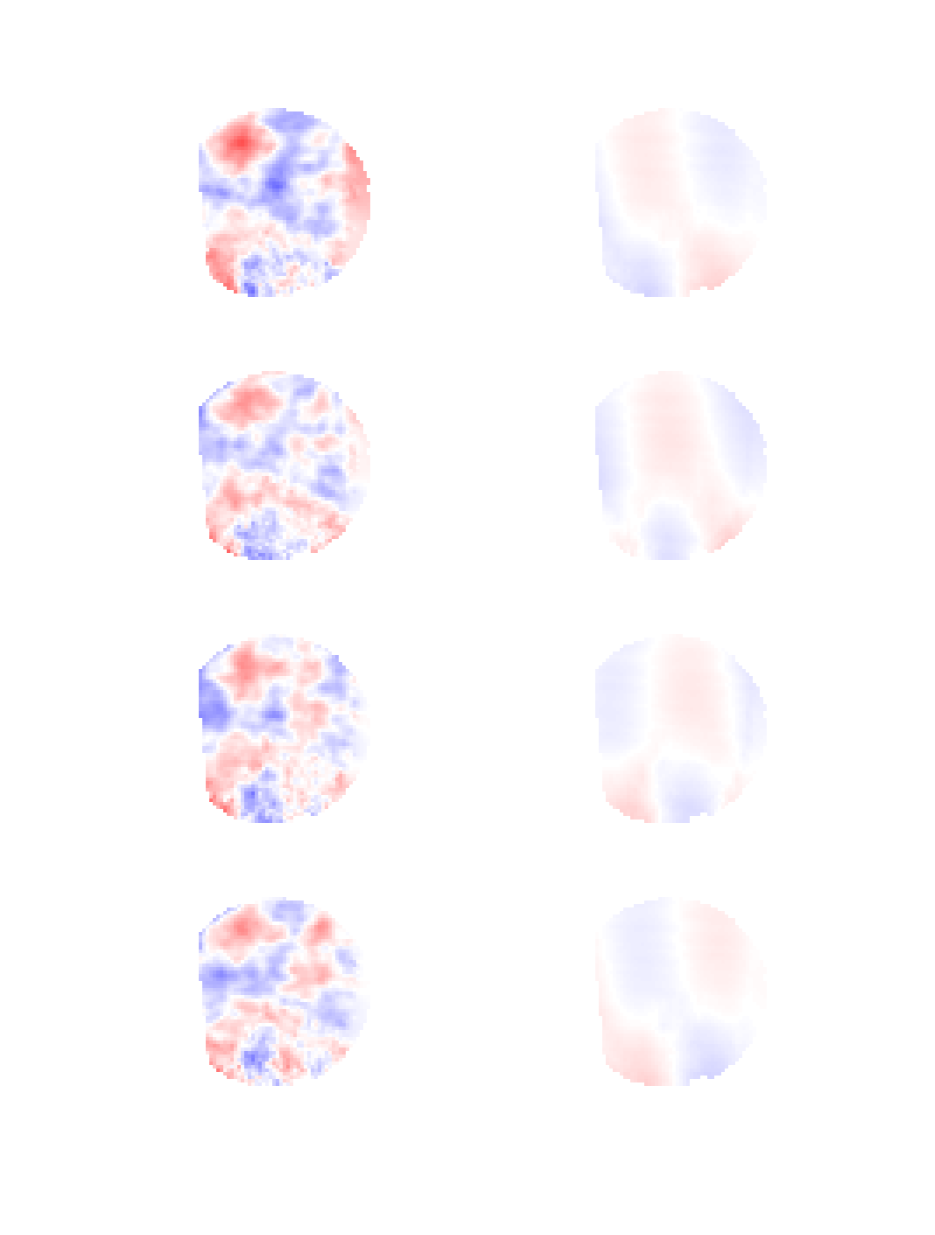
\includegraphics{../matlab/06_single_sensor_filtering/filter_temporal_bandpass.eps}
 \caption{Measured wavefronts filtered at the blade-passing frequency (532$\pm$10 Hz).  The left column is band-stop filtered while the right is band-pass filtered.}
 \label{fig:06_filter_temporal_bandpass}
\end{figure}
The figure shows several wavefront frames of measured data acquired in the Notre Dame White Field wind tunnel and presented previously in Chapter \ref{chap:03_optical_acoustics} (see Figure \ref{fig:03_tunnel_comparison}) that are band-stop filtered in the left column and band-pass filtered in the right column.
The flow is from right-to-left and the band-pass filtered wavefront clearly shows upstream-moving optical disturbances (moving left-to-right against the flow direction) associated with acoustic duct modes traveling upstream from the fan.
On the other hand, the band-stop filtered wavefronts on the left of Figure \ref{fig:06_filter_temporal_bandpass} show much slower-moving optical disturbances that are in general moving in the direction of the flow.
In particular, the downstream-moving disturbances on the left side of Figure \ref{fig:06_filter_temporal_bandpass} have the appearance of boundary-layer aero-optical disturbances, with a scale on the order of the boundary-layer thickness.

Note that for filters that operate in one dimension, the filters were applied over both positive and negative frequencies to the n-dimensional Fourier transform in order to preserve the direction of travel of the signal.
This also allowed several filters to be applied in series without having to perform a Fourier and inverse Fourier transform for each successive filter.
Temporal filters are also used in sizing and/or designing adaptive optics systems \cite{Greenwood-1977-aWDqUh6C} for example.
A low-pass filter with a cutoff at the bandwidth of either a fast-steering or deformable mirror is often used to define the signal that the system needs to reject \cite{Whiteley-2007-bHbWRWUu}.
A control system may need to have the bandwidth reduced in order to keep a mirror’s travel within limits \cite{Madec-2012-YJ8eWhPB}, while a high-pass filter would inform designers of the remaining optical aberrations that cannot be corrected.

\section{Upstream/Downstream Moving}
\label{chap:06_up_down_filter}
In the preceding section, filters based on temporal frequency only were discussed. In this section, another filtering approach is presented in which signals are identified based on their dispersion velocity.
For the filtering of upstream and downstream moving optical disturbances a logistic function was chosen,
\begin{equation}
 f(x) = \frac{1}{1+\exp\{-kx\}} \textrm{.}
 \label{eqn:06_logistic}
\end{equation}
This function was then expanded into two-dimensions ($x$ and $t$).
For a filter that removes disturbances moving against the direction of flow, the filter should ideally return a value of one in both the first and third quadrants and zero otherwise when plotted in a graph of temporal versus spatial frequency.
To accomplish this, the logistic curve in each dimension was scaled and offset to output values between negative one and positive one,
\begin{equation}
 G_t(f) = \frac{2}{1+\exp\{-k_tf\}}-1
 \label{eqn:06_logistic_time}
\end{equation}
and
\begin{equation}
 G_x(\xi_x) = \frac{2}{1+\exp\{\pm k_x\xi_x\}}-1 \textrm{,}
 \label{eqn:06_logistic_space}
\end{equation}
where $\pm$ determines whether the filter is designed to act on upstream-traveling disturbances ($+$) or downstream-traveling ($-$).
These two gain functions are then multiplied together and scaled to output values between zero and one,
\begin{equation}
 G(\xi_x,f) = \frac{(G_t\cdot G_x)+1}{2} \textrm{.}
 \label{eqn:06_up_down_filter}
\end{equation}
As the values of $k_x$ and $k_t$ go to infinity an ideal filter is obtained.
In a plot of the gain with the horizontal spatial frequency on the x-axis and the temporal frequency on the y-axis, an ideal filter for obtaining only the downstream traveling disturbances would have a gain of one in the first and third quadrants, zero in the second and fourth quadrants, and a value of $1/2$ when either frequency is zero.
The value of $1/2$ would equally split the component of a disturbance that is neither traveling upstream or downstream between the two directions.

The multidimensional spectrum using an ideal upstream-moving filter on the synthetic wavefront is shown in Figure \ref{fig:06_filter_downstream} alongside the spectrum of the unfiltered wavefront.
\begin{figure}
 \centering
 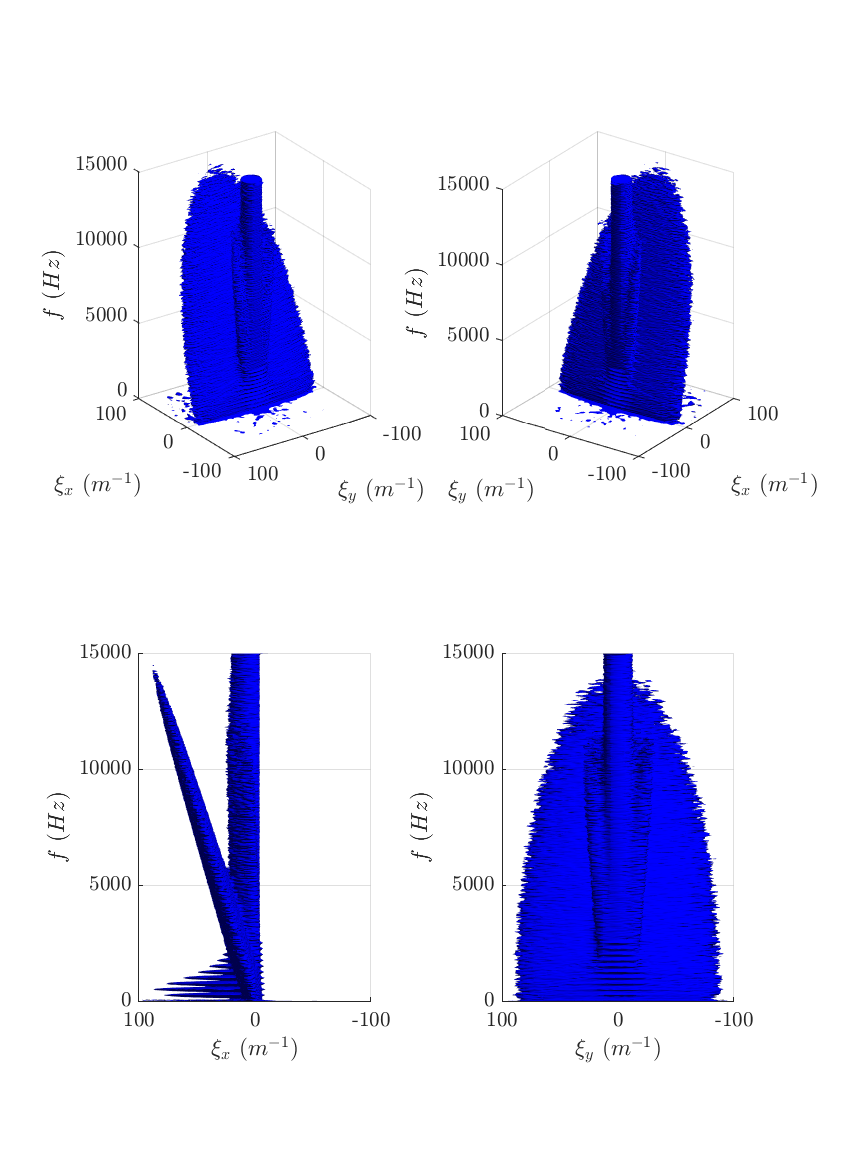
\includegraphics{../matlab/06_single_sensor_filtering/filter_downstream.eps}
 \caption{Multidimensional spectral isosurface of the synthetic wavefront with a downstream filter in place.}
 \label{fig:06_filter_downstream}
\end{figure}
All of the upstream traveling disturbances are removed and the disturbances at the stream-wise spatial frequency $\xi_x=0$ m$^{-1}$ are significantly reduced.
Some of the stationary modes (the vertical cylinder along $\xi_x=0$ and $\xi_y=0$) remain while only the acoustic and vibration signals that are propagating in the direction of flow remain.
The aero-optical signal from the boundary layer is clipped slightly at $\xi_x=0$ due to the spatial width of the signal.
The ratio of the time-averaged spatial-RMS of the filtered signal when compared to the aero-optical only signal was 1.24 while the unfiltered ratio was 1.53.
When the filter was applied to the wavefront with only the aero-optical boundary layer signal present the $\opdrms$ was reduced to 96\% that of the unfiltered wavefront, showing that the filter does not reduce the energy of aero-optical signals convecting with the flow.
Hence, this filter method will retain any disturbance that is traveling in the direction of flow.
Even with an ideal filter there is some slight attenuation of the aero-optical signal due to signal having some spectral width that crosses into upstream-moving portion of the dispersion plot.


\section{Velocity Filtering}
\label{chap:06_velocity_filter}
For a nondispersive medium such as air, flow structures traveling at a given speed have a constant slope on a multidimensional spectral plot.
A plane in the multidimensional spectral plot can therefore be used to measure a flow structure's velocity in both $x$ and $y$-directions.
The distance from any given point in the multidimensional spectral space to a plane described by the velocities $u_x$ and $u_y$ can be computed by
\begin{equation}
 d = \frac{|u_x\xi_x+u_y\xi_y-f|}{\sqrt{u_x^2+u_y^2+1}} \textrm{.}
 \label{eqn:06_dist_point_2_plane}
\end{equation}
Equation \ref{eqn:06_dist_point_2_plane} above can therefore be used to construct a low-pass or high-pass filter that retains only disturbances that are traveling at that velocity, or to exclude those disturbances,
\begin{equation}
  G(d) = \frac{1}{\sqrt{1+\left(\frac{d}{d_c}\right)^{\pm2n}}} \textrm{.}
  \label{eqn:06_butterworth_velocity}
\end{equation}
where $d_c$ is the cutoff distance from the plane defined by the velocities $u_x$ and $u_y$.
Because of differences in the temporal and spatial sample rates of several orders of magnitude, the filter function employed in this research used frequencies that have been normalized by the sample rate.

An example of a low-pass velocity-filter applied to the synthetic wavefront generated in Chapter \ref{chap:05_synthetic} is shown in Figure \ref{fig:06_filter_velocity}.
\begin{figure}
 \centering
 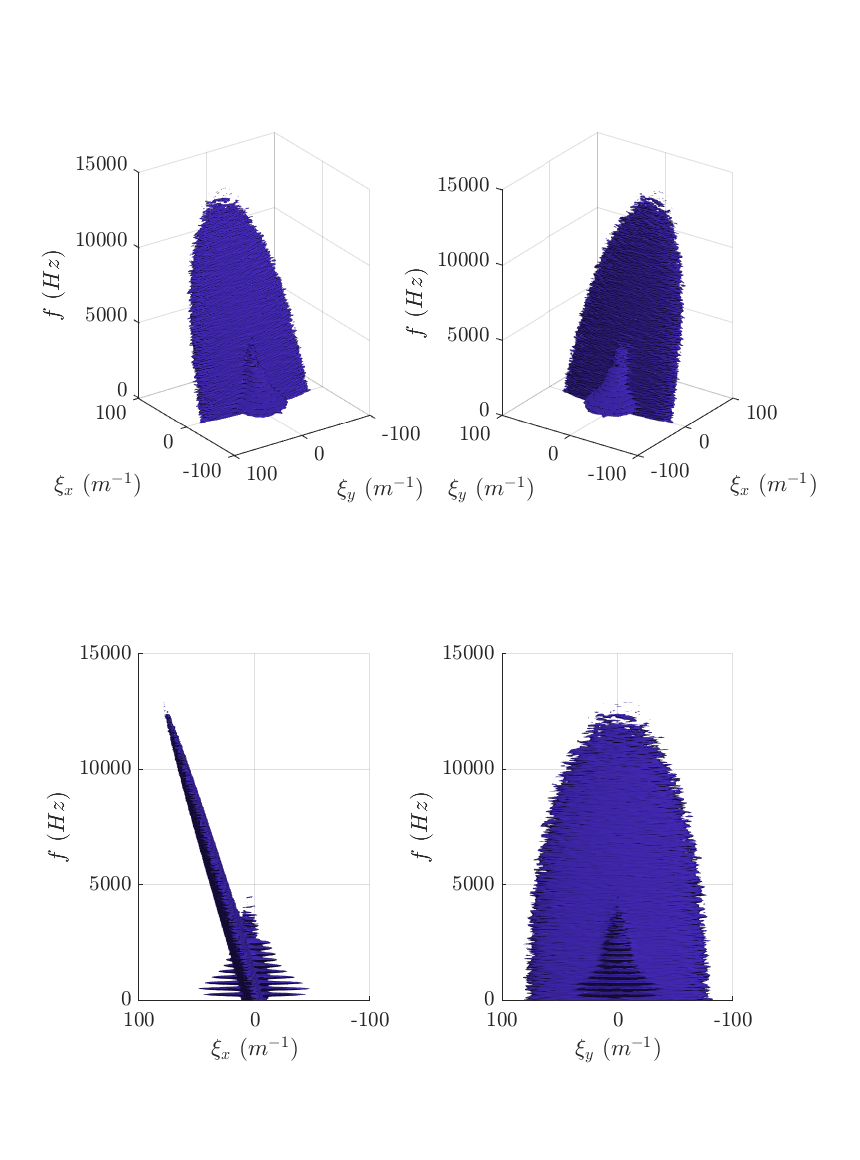
\includegraphics{../matlab/06_single_sensor_filtering/filter_velocity.eps}
 \caption{Multidimensional spectral isosurface of the synthetic wavefront with a low-pass velocity-filter in place.}
 \label{fig:06_filter_velocity}
\end{figure}
The filter was constructed for a $u_x$ set at the mean boundary-layer velocity, and $u_y$ set to zero.
The values of the other two filter parameters were selected as $d_c=1/80$, and $n=1$, which were chosen in a trial-and-error process in which values were chosen, the filtered multidimensional spectrum was computed, and refinements to the parameter values were made based on how well the filtered spectrum captured just the boundary-layer signal.
Figure \ref{fig:06_filter_velocity} shows that, using these filter parameters, the  velocity-filtered multidimensional spectrum successfully retains primarily only the aero-optical signal with some additional low-frequency content from the blade-passing frequency and harmonic disturbances as well as some stationary and acoustic disturbances.
The ratio of the $\opdrms$ relative to that of the aero-optical-only signal went from 1.53 in the unfiltered case to 1.01 in the filtered case, showing that the velocity filter has filtered out a substantial amount of noise and other unrelated signals from the aero-optical signal of the boundary layer, which is presumed to be the objective of the measurement.
As such, this method can provide a very effective way to quickly estimate the $\opdrms$ of a convecting aero-optical disturbance in a noise-contaminated wavefront.

Another use of the velocity filter is measuring the speed of a broadband convecting disturbance such as the aero-optical signal of a boundary layer.
This can be accomplished by applying a series of low-pass velocity filters to the multidimensional spectrum of the wavefront along with a high-pass radial frequency filter to remove a significant portion of the stationary modes and acoustic cone,
\begin{equation}
  S_{xx,f}(\xi_x,\xi_y,f) = S_{xx}(\xi_x,\xi_y,f) G_v^2 G_\rho^2 \textrm{,}
  \label{eqn:06_velocity_filter_measurement}
\end{equation}
where $G_v$ is the velocity filter and $G_\rho$ is the radial frequency ($\xi_rho^2 = \xi_x^2+\xi_y^2$) filter.
Once the wavefront has been filtered in multidimensional spectral space, the total power remaining in the filtered spectrum can be calculated,
\begin{equation}
  P = \sum (S_{xx,f}\prod{\overrightarrow{f_s}}) \textrm{.}
\end{equation}
The average convective velocity of the structure is then given by the filter parameters that produce the maximum power in the filtered signal.

This velocity finding procedure described in the preceding paragraph was tested on the synthetic wavefront generated in Chapter \ref{chap:05_synthetic}, which had a known boundary-layer mean velocity.
The results of the velocity finding analysis are shown in Figure \ref{fig:06_filter_velocity_measure}, which shows the power in the filtered signal as a function of the $u_x$ parameter using in the velocity filter component of Equation \ref{eqn:06_velocity_filter_measurement}.
\begin{figure}
 \centering
 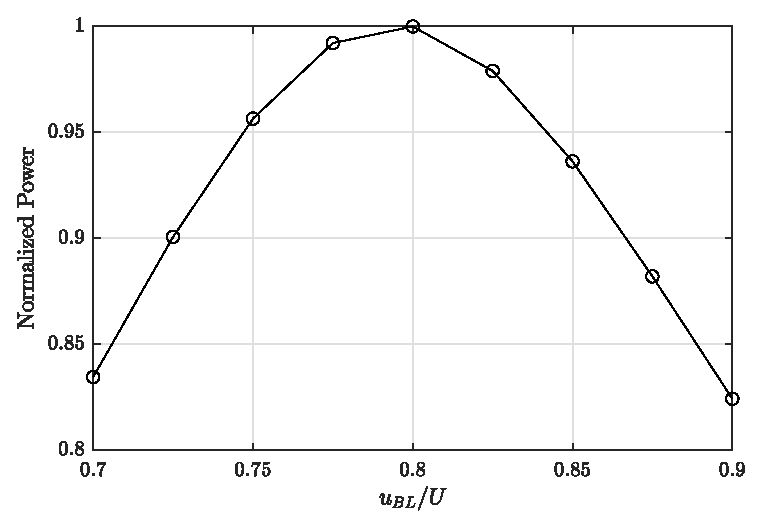
\includegraphics{../matlab/06_single_sensor_filtering/filter_velocity_measure.eps}
 \caption{Boundary layer velocity measurement of the synthetic wavefront using a combination of a low-pass velocity filter and a high-pass radial frequency filter. The maximum value at $u_{BL}/U=0.8$ corresponds with the actual value used in the creation of the synthetic wavefront.}
 \label{fig:06_filter_velocity_measure}
\end{figure}
The low-pass velocity filter used the same parameters as used previously except that $u_x$ was varied and the high-pass radial frequency filter used a cutoff value of 0.1 with an order of $n=2$.
The radial frequency, $\xi_\rho$, was normalized by the spatial sampling rate.
In this case, the boundary layer speed was determined to be 163 m/s which corresponds to the design velocity of the synthetic signal of $0.8U$.
For signals where the mean-velocity component of the aero-optical signal is not aligned with either the horizontal or vertical axis, both velocity components can be varied in the velocity filter.
This produces a three-dimensional surface of filtered signal power as a function of $u_x$ and $u_y$ in the velocity filter, where the velocity components of the moving signal are given by the maximum power of the surface.
An example of this method is shown in Figure \ref{fig:06_filter_velocity_real}, which was computed using experimental wavefront data acquired in the White Field wind tunnel at M=0.5.
\begin{figure}
 \centering
 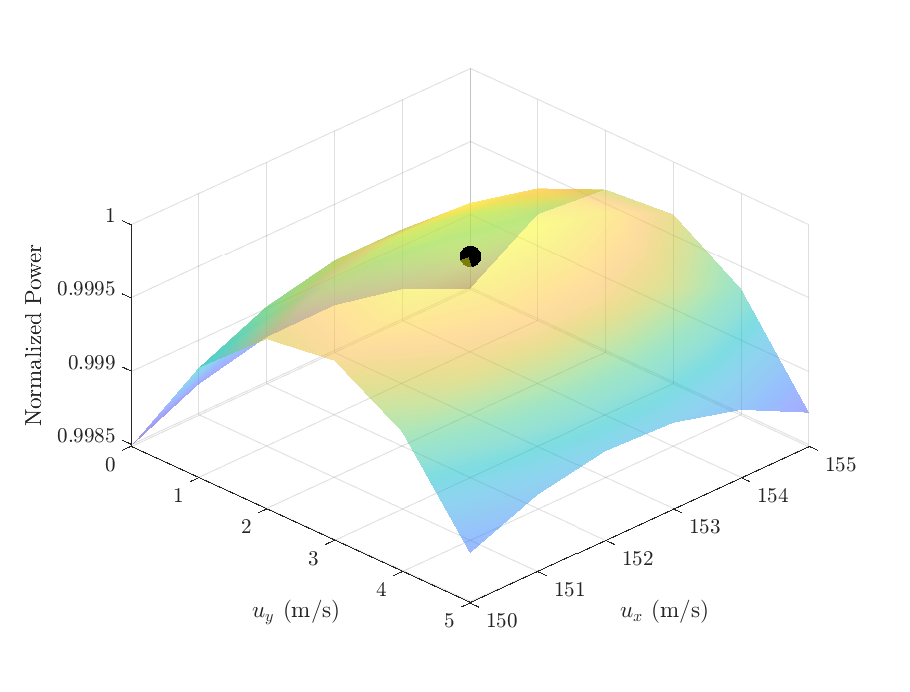
\includegraphics{../matlab/06_single_sensor_filtering/filter_velocity_real.eps}
 \caption{Velocity low-pass filter used to determine the mean disturbance velocity of measured data presented in Figure \ref{fig:04_dispersion_3d}.  The velocity in the x-direction was measured to be 152 m/s and 3 m/s in the y-direction.}
 \label{fig:06_filter_velocity_real}
\end{figure}
In this case the same filtering parameters were used as the synthetic case except the distance cutoff was $d_c=1/40$ and both $u_x$ and $u_y$ were variables.
The velocity components of the boundary-layer optical disturbances determined from Figure \ref{fig:06_filter_velocity_real} are 152 m/s in the x-direction and 3 m/s in the y-direction.
This boundary-layer velocity is approximately 0.85 times the freestream velocity when compared to the pitot probe measurement of the free-stream velocity, which is very close to the accepted speed of the optically-aberrating structures in a boundary-layer flow \cite{Gordeyev-2014-jcJndkHM}.
The overall flow angle of the boundary-layer with respect to the orientation of the measurement beam was approximately $1.1^\circ$.

\section{Baseline Spectrum}
\label{chap:06_baseline}
If all of the narrow-band temporal signals in a data set can be assumed to be measurement contamination that needs to be filtered out, a method for calculating the baseline of the spectrum provides a simple way of filtering a portion of the signal contamination.
For example, during analysis of Raman spectra, the baseline spectra must often be removed \cite{Schulze-2012-GmyAqzC7}.
This task is often performed manually which has resulted in a number of attempts to create automated techniques to estimate the baseline spectra \cite{Mosier-Boss-1995-keK3ckUN, Schulze-2005-QkUeywxD, Schulze-2012-GmyAqzC7, Zhao-2007-HAc6j8Wb}.
One of those techniques \cite{Schulze-2012-GmyAqzC7}, a small-window moving-average based, fully automated baseline estimation method was used in this research.
For this method, at each spatial frequency location, the baseline spectrum was computed along the temporal axis.
This process estimates the baseline spectrum, $\mathbf{b}$, from the measured spectrum, $\mathbf{m}$,
\begin{equation}
  \mathbf{m} = (\mathbf{b}+\mathbf{x})*\mathbf{p}+\mathbf{n} = \mathbf{b}*\mathbf{p}+\mathbf{x}*\mathbf{p}+\mathbf{n} \textrm{,}
\end{equation}
where $\mathbf{x}$ is a pure or underlying signal vector, $\mathbf{p}$ is an instrumental blurring function, $\mathbf{n}$ is measurement noise, and $*$ is convolution operator.

Figure \ref{fig:06_filter_baseline}, shows the multidimensional spectrum of an unfiltered measurement (top left) and its estimated baseline spectrum (top right).
\begin{figure}
  \centering
  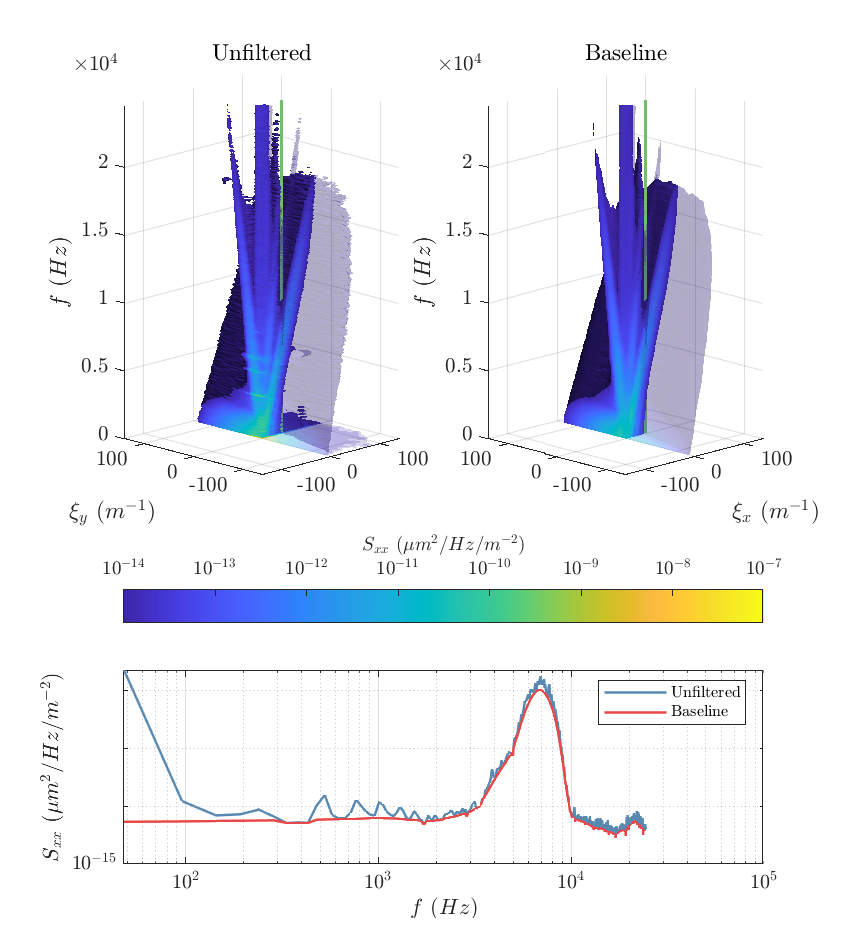
\includegraphics{../matlab/06_single_sensor_filtering/filter_baseline.eps}
  \caption{Baseline spectrum estimation. The top left plot shows the unfiltered multidimensional spectrum and the baseline spectrum on the top right. The green line in each of these plots represents the location at which the spectra in the bottom plot is shown.}
  \label{fig:06_filter_baseline}
\end{figure}
The bottom plot of the figure shows the unfiltered and baseline spectra along the green line in the two multidimensional spectral plots.
The total power of the signal has been reduced by $~71\%$ with all of the narrow-band signals removed.
A large portion of this signal removal is the very low temporal frequency components.
The blade-passing frequency and harmonics are completely removed but the broadband acoustic duct-modes remain intact.
The peak of the boundary-layer signal is reduced slightly as well as the high frequency fluctuations.

\section{Basic Filter Summary}
Three different basic wavefront filters were shown and discussed in this chapter.
The temporal filter is most useful when filtering out a frequency band of optical noise.
Besides filtering out optical noise, band-pass filters can be used to analyze a wavefront over a narrow-band to examine the optical aberrations at specific frequencies that significantly contribute to the overall optical disturbance; for example, as was shown in Chapter \ref{chap:03_optical_acoustics}, band-pass filters along with an implementation of an acoustic mode-marching method can help determine with some confidence that a narrow-band signal is likely to have been created by the wind-tunnel fan and can be removed.

Filters that separate upstream and downstream-moving disturbances are useful to filter out the optical contamination that comes from acoustic signals that are traveling upstream from a wind-tunnel fan.
These filters would also be useful for separating out an aero-optical signal that has a broad range of velocities that can occur in a span wise measurement of a boundary layer.
The velocity filter is the most useful for isolating the aero-optical portion of a wavefront measurement given the aero-optical signal has a fairly narrow and constant velocity range.
This filter also can be used to measure the speed associated with an optical disturbance in both x and y-directions.

The spectral baseline provides a simple way of removing all of the narrow-band signals with slight attenuation to the broadband signals.
The broadband acoustic and stationary modes remain but could be filtered with via other techniques such as using a velocity filter.
Narrow-band features that are not likely to be environmental contamination could be easily added back in.

\section{Multiple Sensor Filtering of Optical Wavefronts}
In the previous sections, methods of filtering optical wavefront corruption by applying a variety of filters to the wavefront in the multidimensional spectral domain were investigated.
These techniques involve only data from the optical wavefront itself and user knowledge and experience to obtain filtered data.
When additional data are available, such as from microphones or accelerometers, a targeted filter approach becomes possible.

This kind of approach is described in a previous study \cite{DeLucca-2014-RAJvGdv7} in which a combination of linear stochastic estimation (LSE) and spectral proper orthogonal decomposition (SPOD) was used to remove vibration related contamination from aero-optical wind-tunnel measurements.
This process along with optical tip and tilt removal showed approximately an 85\% removal of contamination in the measured $\opdrms$ by using accelerometer measurements to remove vibration effects from optical wavefront measurements.

Finally, this chapter concludes by showing results produced by applying the LSE-SPOD filter to experimental wavefront data acquired in the White Field wind tunnel, both by itself and in combination with the filters described in Chapter \ref{chap:06_single_filter}. The objective of the filtering approaches shown was to filter out contamination from the aero-optical signal produced by the boundary layer on the measurement aperture. The performance of the various filtering methods are compared and recommendations for the best filtering approach are given.

\subsection{Optical Tip and Tilt}
Although they are usually not employed in aero-optical investigations, Zernike polynomials have been traditionally used for modal decomposition of the optical aberrations of an optical system \cite{Born-1965-HHGYgjdH}.
These polynomials are defined on the unit circle and form a set of orthogonal functions,
\begin{equation}
  Z_n^m(\rho,\theta) = R_n^m(\rho)\cos(m\theta)
  \label{eqn:07_zernike}
\end{equation}
where $R_n^m(\rho)$ is the radial basis function and $\cos(m\theta)$ is the angular basis function.
For values of $-m$ the angular basis function becomes $\sin(m\theta)$.
The radial basis functions are developed from Jacobi polynomials but for purposes of this study, only a few simple ones will be used.
An optical wavefront can be represented by a summation of Zernike polynomials multiplied by their corresponding coefficients
\begin{equation}
  \wf = \sum Z_ja_j \textrm{.}
  \label{eqn:07_zernike_coeff}
\end{equation}

The Noll naming scheme is a method of organizing the Zernike polynomials into a single notation of $Z_j$, along with normalizing each polynomial to have a spatial RMS equal to one \cite{Noll-1976-HHKzd88f}.
The first three of these using the Noll naming scheme are piston, tip, and tilt.
Piston is simply the average $\opd$ value of the wavefront
\begin{equation}
  Z_1 = 1 \textrm{.}
  \label{eqn:07_zernike_1}
\end{equation}
Tip and tilt are the best planar fit to the $\opd$ along the x-axis and y-axis respectively where tip is
\begin{equation}
  Z_2 = 2\rho\cos\theta \textrm{,}
  \label{eqn:07_zernike_2}
\end{equation}
and tilt is
\begin{equation}
  Z_3 = 2\rho\sin\theta \textrm{.}
  \label{eqn:07_zernike_3}
\end{equation}
Once the coefficients for these modes are solved for they can be removed from the original wavefront, $WF$:
\begin{equation}
  WF^F = WF-\sum Z_ja_j \textrm{.}
\end{equation}

\subsection{LSE-SPOD}
The LSE-SPOD technique starts with performing SPOD on the primary data set and then using the Fourier transforms of the additional sensor data to perform a filtering operation.
The spectral proper orthogonal decomposition technique is described in detail by Schmidt and Colonius \cite{Schmidt-2020-m2emACkX}.
A schematic of the SPOD algorithm is shown in Figure \ref{fig:07_spod_algorithm}.
\begin{figure}
  \centering
  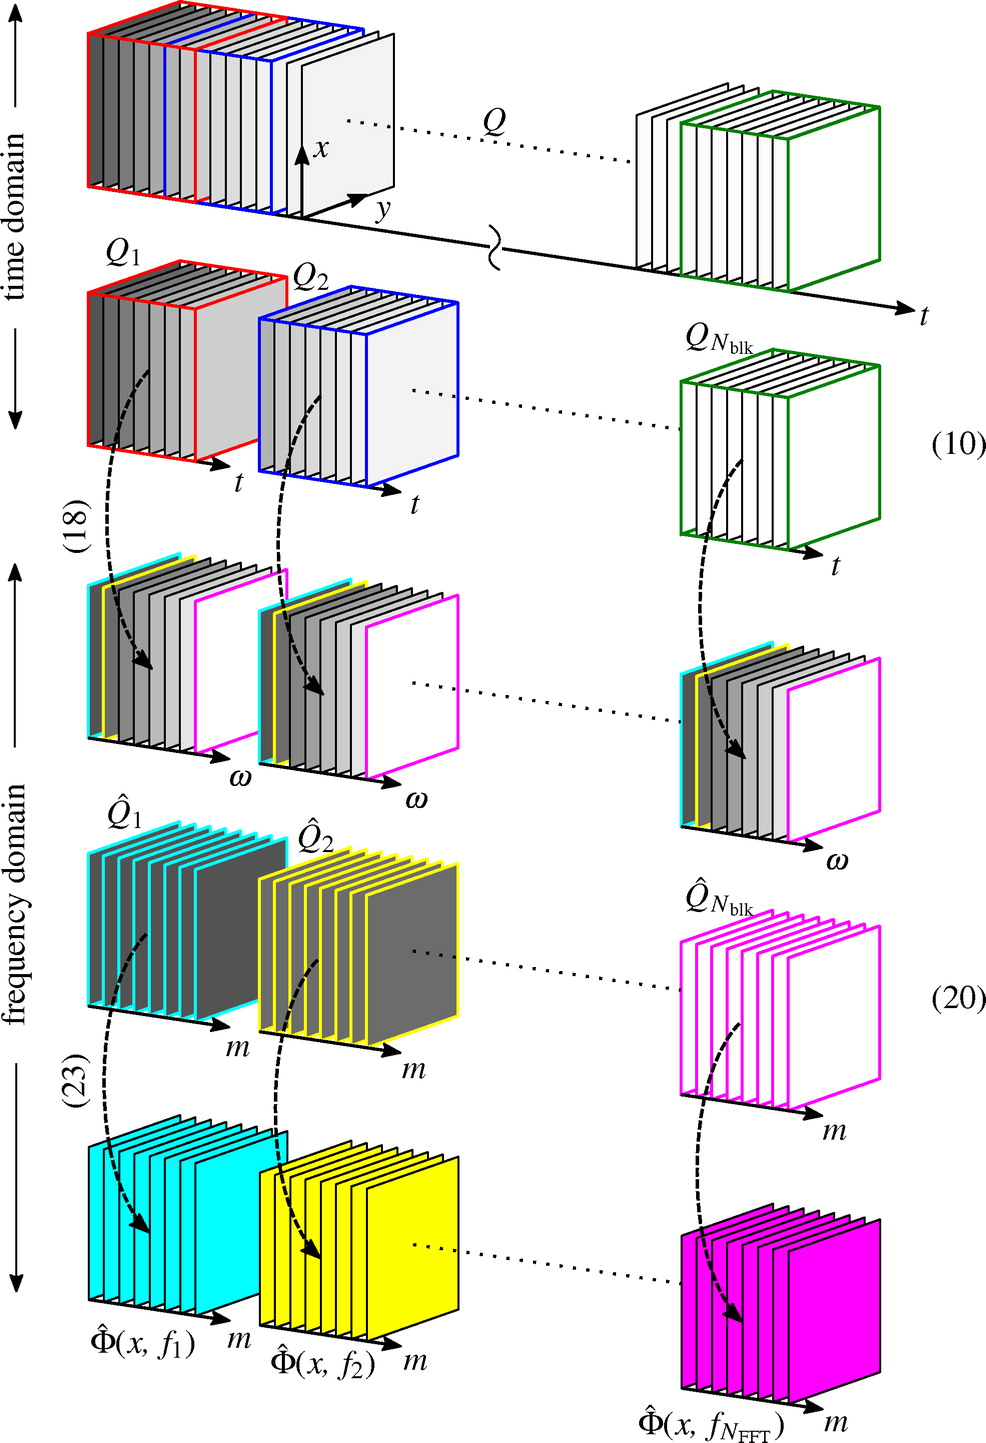
\includegraphics{../other-sources/schmidt_2020_figure_01.jpeg}
  \put(-20,235){\fcolorbox{white}{white}{\footnotesize(\ref{eqn:07_data_block})}}
  \put(-230,210){\rotatebox{90}{\fcolorbox{white}{white}{\color{white}{empt}}}}
  \put(-20,102){\fcolorbox{white}{white}{\footnotesize(\ref{eqn:07_frequency_block})}}
  \put(-231,69){\rotatebox{90}{\fcolorbox{white}{white}{\footnotesize(\ref{eqn:07_pod_01}-\ref{eqn:07_pod_04})}}}
  \caption{Schematic of the SPOD algorithm (taken from \cite{Schmidt-2020-m2emACkX}). The numbers in parentheses denote the equations used.}
  \label{fig:07_spod_algorithm}
\end{figure}
The algorithm begins by separating the original data set, $Q$, into a number of smaller blocks,
\begin{equation}
  Q = \left[
  \begin{matrix}
    \mid & \mid & & \mid \\
    q^{(1)} & q^{(2)} & \cdots & q^{(N)} \\
    \mid & \mid & & \mid
  \end{matrix}
  \right]\textrm{,}\quad Q\in\mathbb{C}^{M\times N}
  \label{eqn:07_data_block}
\end{equation}
where $M$ is the total number of degrees of freedom (number of spatial points times the block length in time) and $N$ is the number of blocks.
Each block is then Fourier Transformed in the temporal dimension or through all dimensions.
Once in the frequency domain the data blocks are then reorganized by creating new blocks of identical temporal-frequencies,
\begin{equation}
  \hat{Q} = \left[
  \begin{matrix}
    \mid & \mid & & \mid \\
    \hat{q}^{(1)} & \hat{q}^{(2)} & \cdots & \hat{q}^{(N)} \\
    \mid & \mid & & \mid
  \end{matrix}
  \right]\textrm{,}\quad \hat{Q}\in\mathbb{C}^{M\times N}
  \label{eqn:07_frequency_block}
\end{equation}
where $M$ is now the number of spatial points times the number of blocks and $N$ is block length in time.
Proper orthogonal decomposition is then performed separately on each temporal-frequency block via either traditional POD
\begin{equation}
  \hat{C} = \frac{1}{N-1}\hat{Q}\hat{Q}^H \textrm{,}
  \label{eqn:07_pod_01}
\end{equation}
\begin{equation}
  \hat{C}W\hat{\Phi}=\hat{\Phi}\hat{\Lambda} \textrm{,}
  \label{eqn:07_pod_02}
\end{equation}
or the method of snapshots,
\begin{equation}
  \hat{Q}^HW\hat{Q}\hat{\Psi}=\hat{\Psi}\hat{\Lambda} \textrm{,}
  \label{eqn:07_pod_03}
\end{equation}
\begin{equation}
  \hat{\Phi}=\hat{Q}\hat{\Psi} \textrm{,}
  \label{eqn:07_pod_04}
\end{equation}
where $H$ denotes the Hermitian transpose, $W$ is a weighting matrix, $\Phi$ is the set of deterministic spatial functions, $\Lambda$ is the eigen-values, and $\Psi$ is the coefficient matrix.

The linear stochastic estimation portion of the technique is described by Adrian \cite{Adrian-1975-VenaZyuv}.
This process uses a linear sum, $L_{ij}$, of additional measurements, $y_j$, to approximate a measured signal, $x_i$,
\begin{equation}
  x_i^{LSE}=L_{ij}y_j \textrm{,}
  \label{eqn:07_lse_01}
\end{equation}
where
\begin{equation}
  L_{ij} = \langle x_iy_k\rangle\langle y_jy_k\rangle^{-1} \textrm{.}
  \label{eqn:07_lse_02}
\end{equation}
When combined with SPOD, the estimation matrix, $L$, becomes
\begin{equation}
  L=(\hat{\Psi}\hat{y}^H)(\hat{y}\hat{y}^H)^{-1} \textrm{,}
  \label{eqn:07_lse_spod_01}
\end{equation}
which allows for an estimated version of the coefficient matrix to be calculated
\begin{equation}
  \hat{\Psi}^E=L\hat{y} \textrm{.}
  \label{eqn:07_lse_spod_02}
\end{equation}
The estimated coefficient matrix contains portions of the original signal that best resemble the additional sensor data.
Assuming that the additional sensor data represents signal contamination of the original signal, a filtered coefficient matrix can be computed from the difference between the original and estimated coefficient matrices.
\begin{equation}
  \hat{\Psi}^F=\hat{\Psi}-\hat{\Psi}^E \textrm{.}
  \label{eqn:07_lse_spod_03}
\end{equation}
A filtered signal, $Q^F$ can be constructed by using the filtered coefficient matrix and the spatial functions,
\begin{equation}
  \hat{Q} = \hat{\Psi}^F\hat{\Phi}^H \textrm{.}
\end{equation}

\subsection{Filtering Experimental Data}
The filtering technique described in the preceding section was applied to the same data sets that were shown in Figure \ref{fig:04_dispersion_mach}, either separately or in combination with the basic filtering methods described earlier in this chapter.
Simultaneous accelerometer and microphone measurements were made alongside the optical wavefront measurements.
The locations of some of the additional sensors are shown in Figure \ref{fig:07_sensor placement} with a CAD drawing of the test section in Figure \ref{fig:07_test_section_mic_accel}.
Table \ref{tab:07_sensor_list} shows a list of the additional sensors including the number designation used in Figures \ref{fig:07_sensor placement} and \ref{fig:07_test_section_mic_accel}, the model of the sensor and preamplifier used as well as a sensor grouping designation.
\begin{figure}
  \centering
  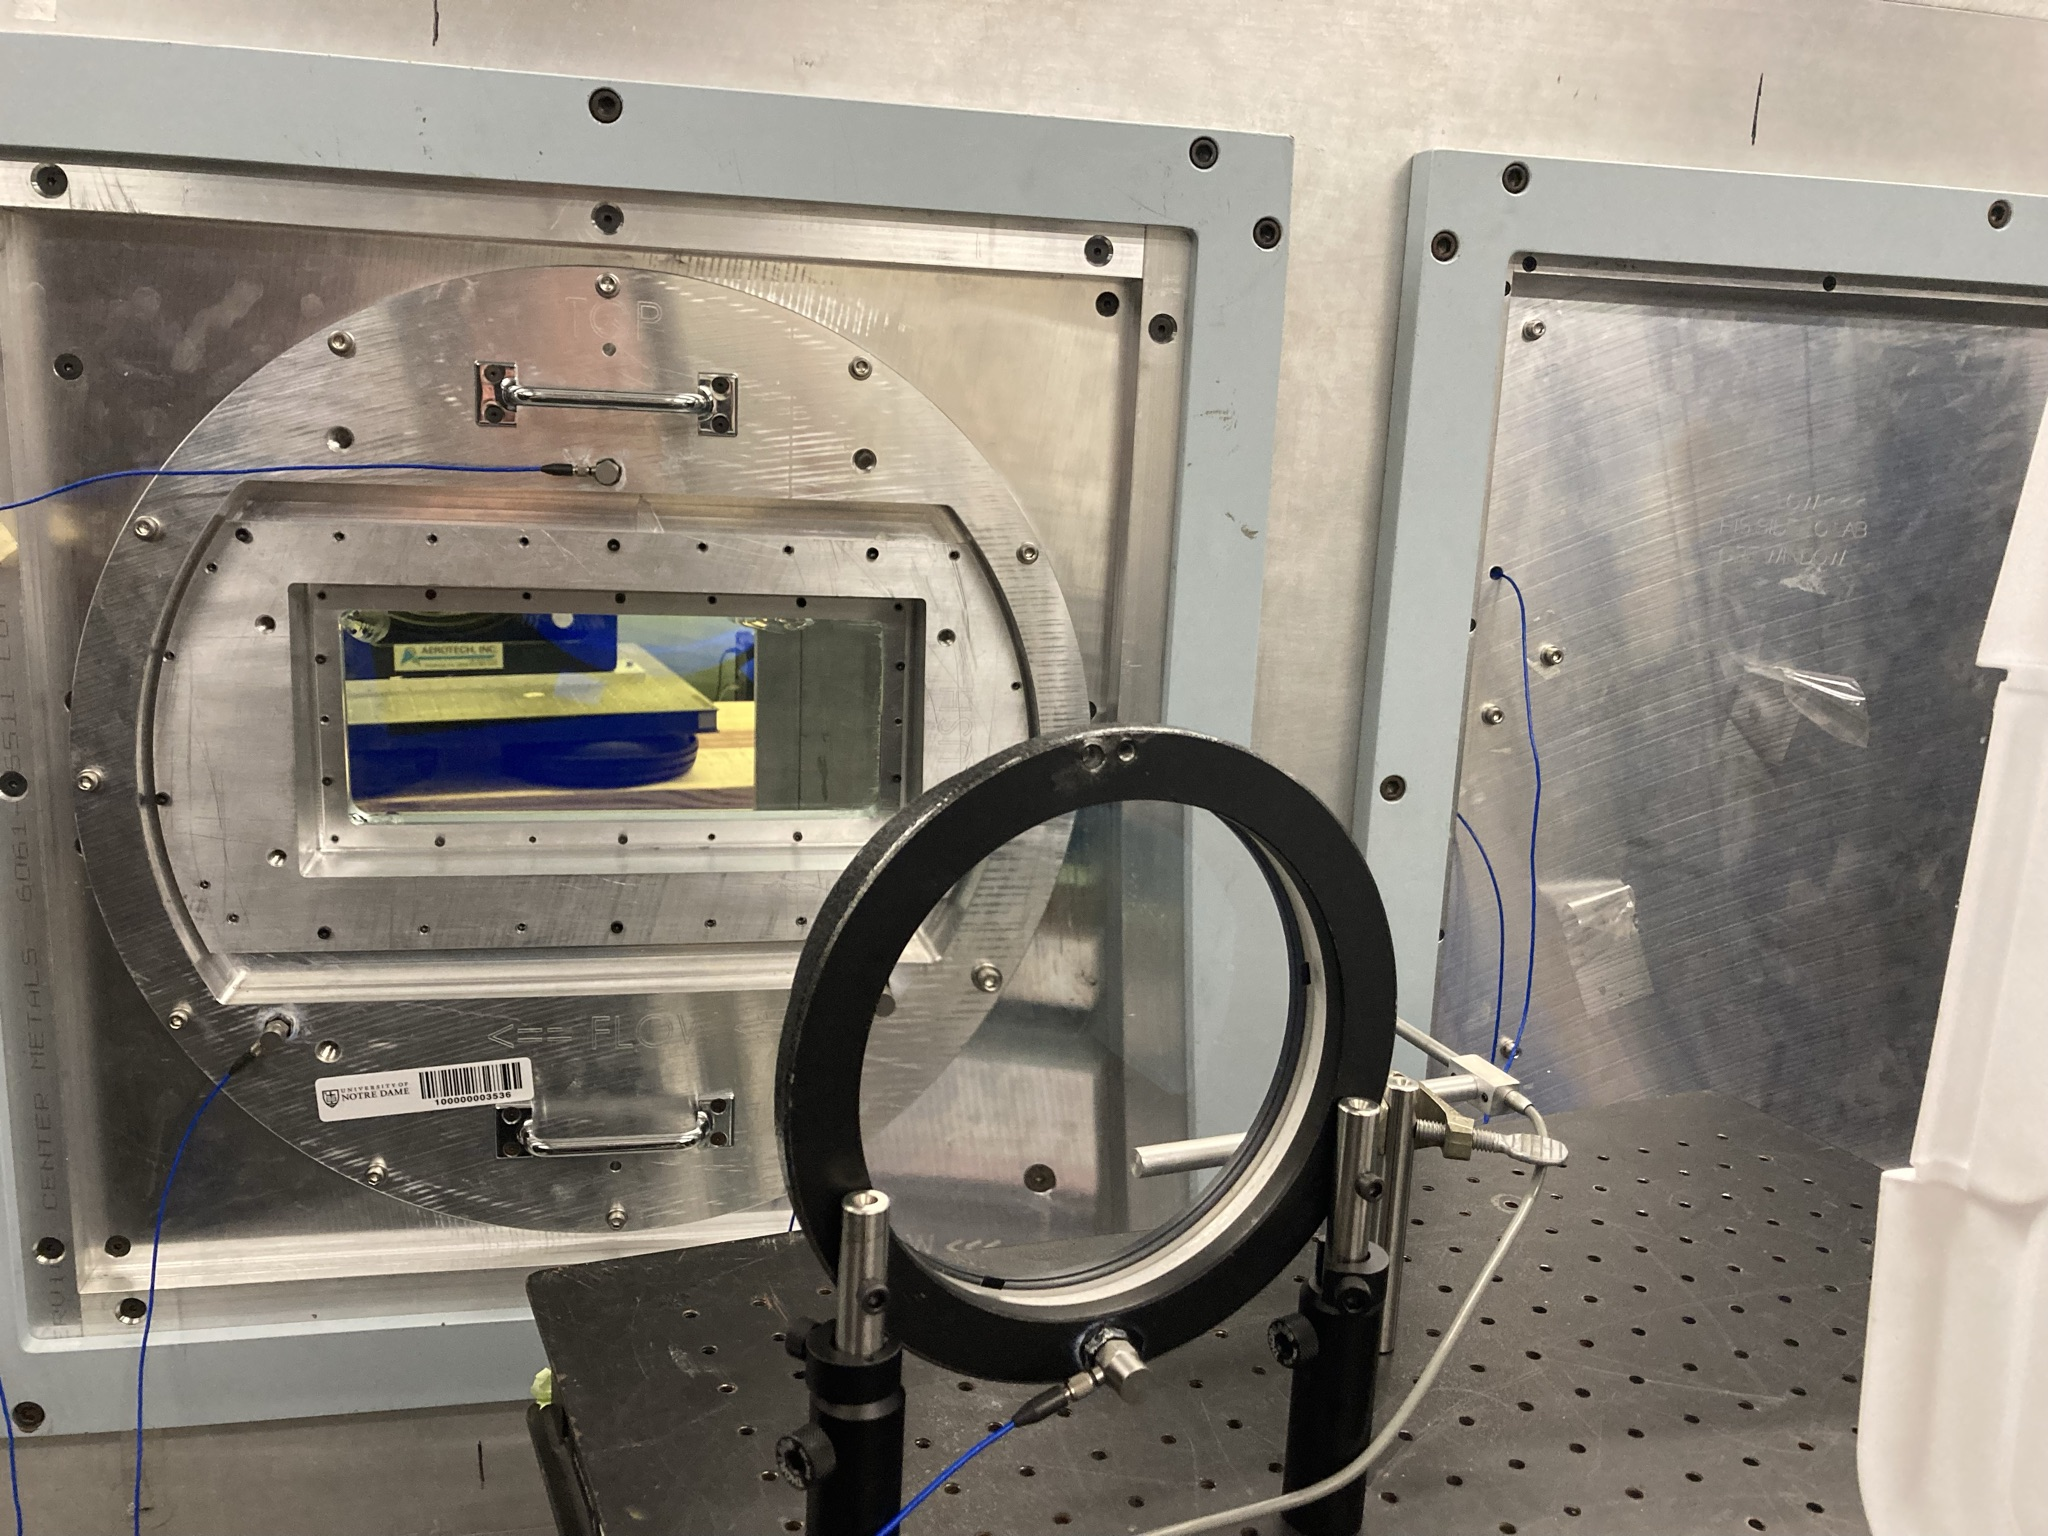
\includegraphics[trim={0 0 5in 3in},clip,width=0.9\textwidth]{../photos/IMG_9655.jpeg}
  \put(-65,120){\circledfill{\large 1}}
  \put(-40,220){\circledfill{\large 3}}
  \put(-50,165){\circledfill{\large 4}}
  \put(-125,40){\circledfill{\large 7}}
  \put(-243,240){\circledfill{\large 8}}
  \put(-180,120){\circledfill{\large 9}}
  \put(-320,110){\circledfill{\large 10}}
  \caption{The locations of some of the additional sensors used in the LSE-SPOD filtering. The sensors are labeled with the sensor numbers, see Table \ref{tab:07_sensor_list}.}
  \label{fig:07_sensor placement}
\end{figure}
\begin{figure}
  \centering
  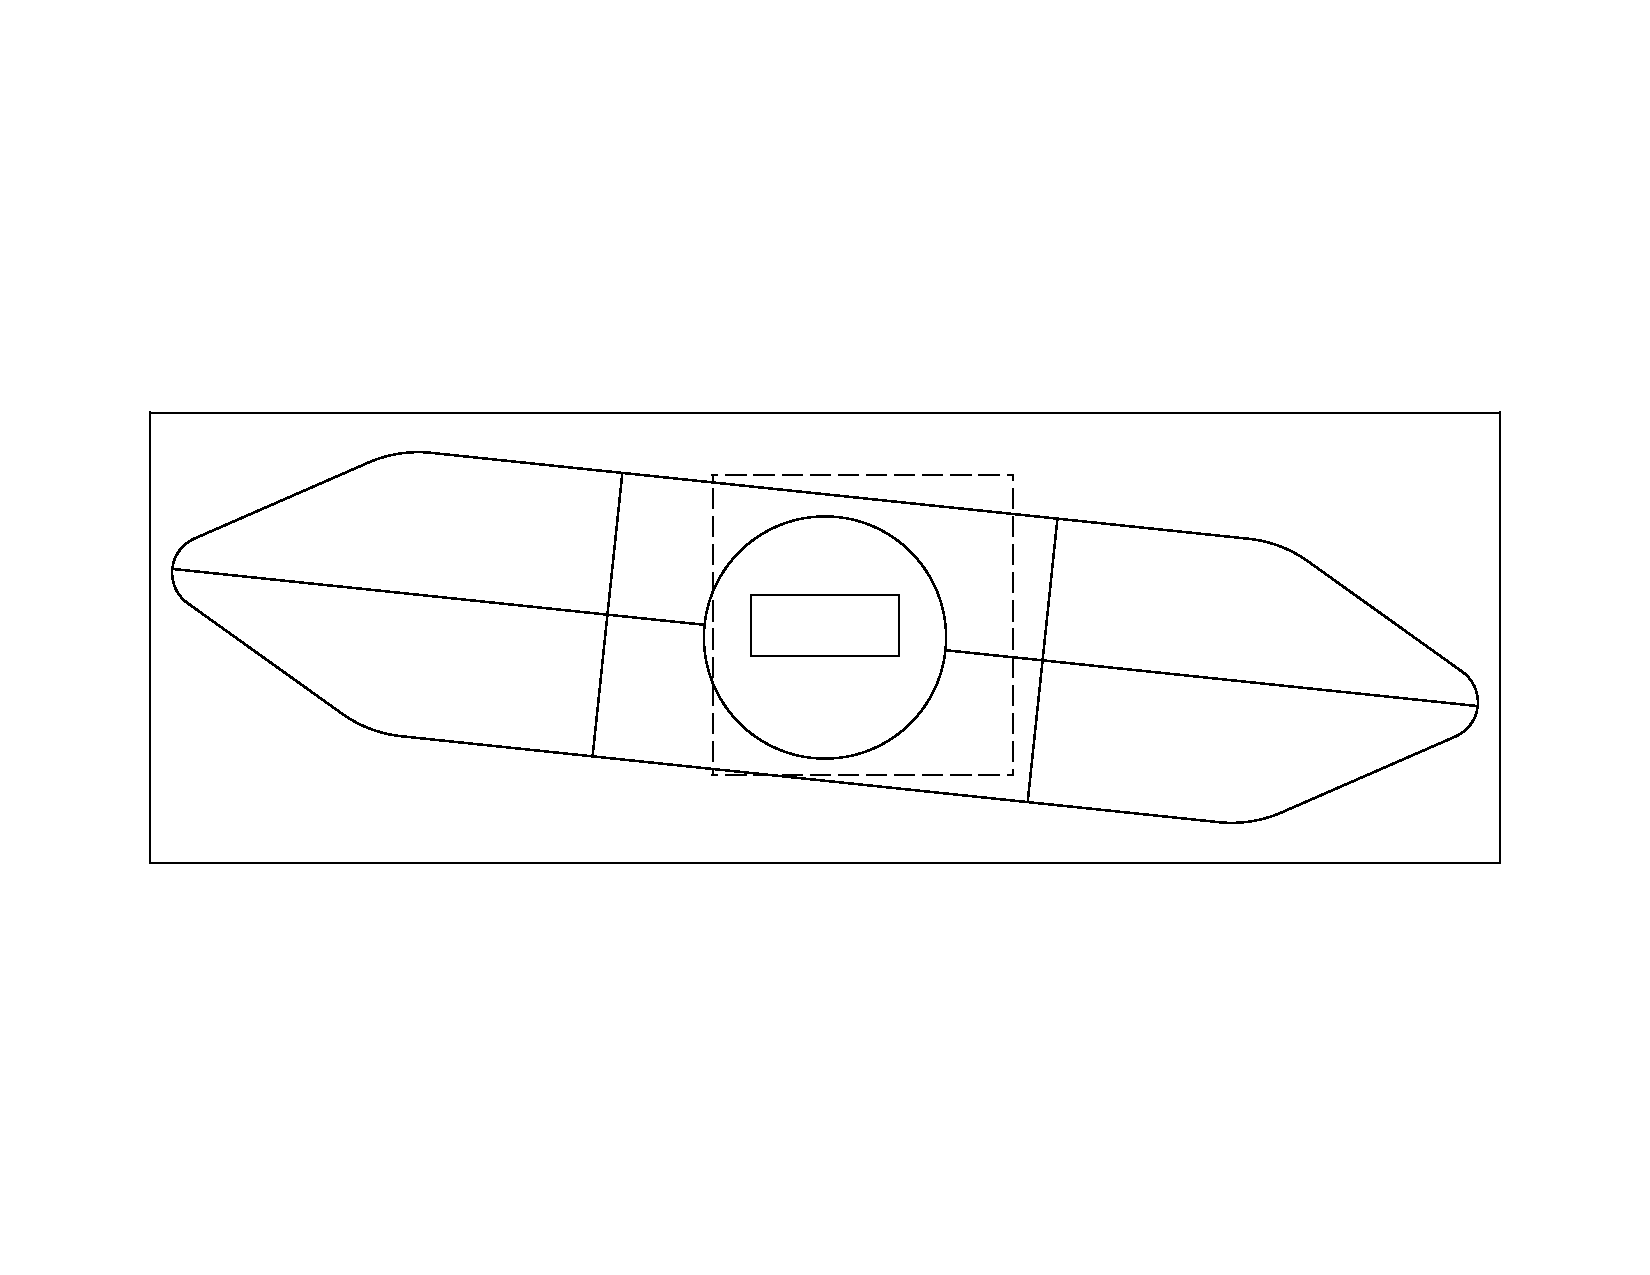
\includegraphics[trim={1in 2.75in 1in 2.75in},clip,width=0.9\textwidth]{../cad/test_section_mic_accel.pdf}
  \put(-272,77){\circled{\large 3}}
  \put(-274,60){\circled{\large 4}}
  \put(-131,61){\circled{\large 5}}
  \put(-133,45){\circled{\large 6}}
  \put(-203,82){\circled{\large 8}}
  \put(-220,46){\circled{\large 9}}
  \put(-188,46){\circled{\large 10}}
  \put(-188,12){\squared{\large 11}}
  \put(-243,100){\squared{\large 12}}
  \put(-140,100){\squared{\large 13}}
  \put(-350,10){\Large Flow $\Longrightarrow$}
  \caption{CAD drawing view of the inside of the test-section with some of the sensor locations labeled. Flow is from left to right. The numbers in the circles are the sensor numbers on the model side of the test-section. The numbers in the square are the sensor numbers opposite of the model side. The dashed line represents the optics window opposite of the model for the beam angle of $90^\circ$. The window was moved up and downstream depending on the beam angle.}
  \label{fig:07_test_section_mic_accel}
\end{figure}
\begin{table}
  \centering
  \caption{Additional sensors used the the LSE-SPOD filtering.}
  \begin{tabular}{c c c c c}
    Channel & Sensor Type & Model & Preamp & Group\\
    \hline \hline
    1 & Microphone & ACO 7016B & B\&K 2690 & Ambient \\
    2 & Microphone & B\&K 4939 & B\&K 2690 & Ambient \\
    3 & Microphone & PCB 103B02 & PCB 483C & Test Section \\
    4 & Microphone & PCB 103B02 & PCB 483C & Test Section \\
    5 & Microphone & PCB 103B02 & PCB 483C & Test Section \\
    6 & Microphone & PCB 103B02 & PCB 483C & Test Section \\
    7 & Accelerometer & PCB 352C33 & PCB 483C & Primary Lens \\
    8 & Accelerometer & PCB 352C33 & PCB 483C & Test Section \\
    9 & Accelerometer & PCB 352C33 & PCB 483C & Test Section \\
    10 & Accelerometer & PCB 352C33 & PCB 483C & Test Section \\
    11 & Accelerometer & PCB 352C33 & PCB 482A22 & Test Section \\
    12 & Accelerometer & PCB 352C33 & PCB 482A22 & Test Section \\
    13 & Accelerometer & PCB 352C33 & PCB 482A22 & Test Section \\
    14 & Accelerometer & PCB 352C33 & PCB 482A22 & Optics Bench \\
    15 & Accelerometer & PCB 352C33 & PCB 482A22 & Return Mirror \\
    16 & Accelerometer & PCB 352C33 & PCB 482A22 & Return Mirror \\
  \end{tabular}
  \label{tab:07_sensor_list}
\end{table}
All of the test-section mounted sensors are shown in their approximate locations in Figure \ref{fig:07_test_section_mic_accel} in a view that is looking at the wind-tunnel model from inside of the test-section with the flow moving from left-to-right.
The dashed box represent the optical window on the opposite side of the tunnel from the model which was moved up or downstream depending on the beam angle relative to the flow.
Sensors 11-13 were attached to this optical window and moved with it.
The picture in Figure \ref{fig:07_sensor placement} was taken from the opposite side of the test-section and model that is shown in Figure \ref{fig:07_test_section_mic_accel} and as such the flow goes from right-to-left.

Two microphones were used for ambient measurement (a ACO 7016B \cite{ACO-Microphones} and a Br\"uel \& Kj\ae r 4939 \cite{Bruel-Kjaer-4939}), four microphones were used for test-section noise measurement (PCB 103B02 \cite{PCB-103B02-C}), and ten accelerometers were located throughout the setup (PCB 352C33 \cite{PCB-352C33-H}).
One of the ambient microphones was mounted to the top of the optics bench facing the test-section and can be seen in Figure \ref{fig:07_sensor placement} just to the right of the primary lens and the other ambient microphone was hanging below the optics bench end towards the test-section.

The test-section microphones were in groups of two either upstream or downstream from the optical beam by about 20-inches, with the upstream microphone locations viewable in Figure \ref{fig:07_sensor placement} (sensors 3 and 4) and shown in Figure \ref{fig:07_test_section_mic_accel}.
The model installed in the test-section represents the outside of an aircraft fuselage with a 5-foot diameter and is angled to account for the aircraft's angle-of-attack (~6$^\circ$) for steady-level-flight at cruise.
This results in the fuselage model being shifted approximately 2-inches higher from the test-section centerline upsteam at the microphone location.
The duct microphones were placed about 2.75-inches from the model centerline.

There were six accelerometers attached to the test-section windows, with three being on each side as shown in Figure \ref{fig:07_test_section_mic_accel}.
The locations of the three accelerometers (sensors 8-10) on the model side can be seen in Figure \ref{fig:07_sensor placement}, the three accelerometers on the other window used the opposite pattern (two high and one low).
The optical window on the far side of the test-section was moved laterally depending on the angle of the beam relative to the flow.
One accelerometer was placed on the primary lens (also shown, sensor 7) and one was placed in the center of the optics bench.
The last two accelerometers were located on the back of the return mirror with one on the top and the other on the side.

\section{Results}
The power-spectra of all of the sensors at the three Mach numbers are shown in Figure \ref{fig:07_sensor_spectra}.
\begin{figure}
  \centering
  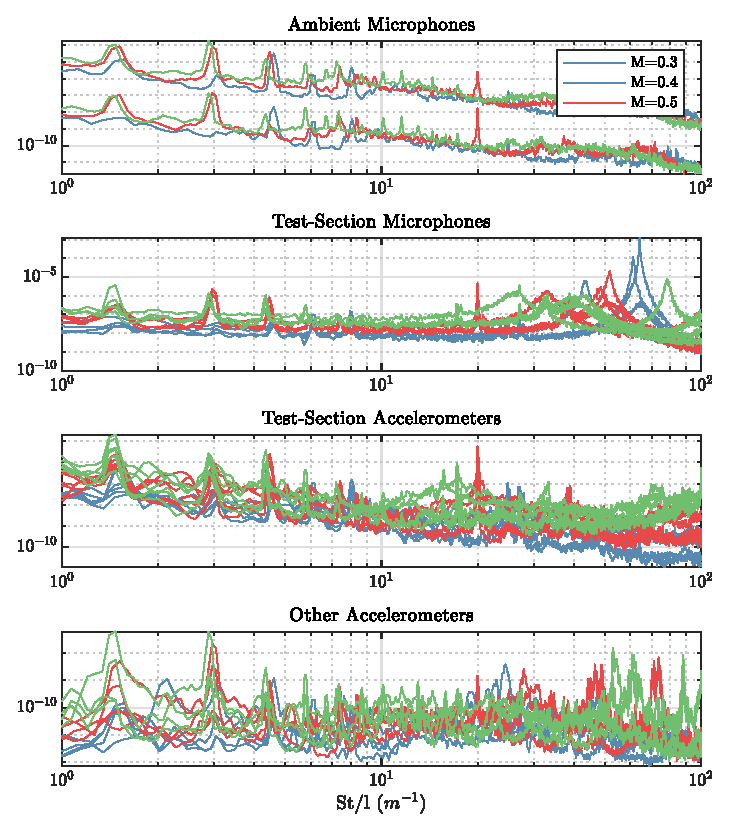
\includegraphics{../matlab/07_multiple_sensor_filtering/sensor_spectra.eps}
  \caption{Power-spectra of the additional sensor measurements at the three Mach numbers tested. The x-axis is in Strouhal number per characteristic length ($St/l$).}
  \label{fig:07_sensor_spectra}
\end{figure}
These plots are presented as Strouhal number per unit characteristic length, since this puts the signals related to the fan blade-passing frequency at the same x-axis location for all three tested wind speeds.
Figure \ref{fig:07_sensor_spectra} also shows the different groups of sensors shown together in separate plots.
The blade-passing frequency for these data sets is at a $St/l$ of approximately 3 $m^{-1}$ with a clear and consistent narrow-band signal at that $St/l$ for all but the $M=0.3$ run, which has a slight increase in signal for some of the sensors.
For the $M=0.5$ case there is an additional strong narrow-band signal at 20 $m^{-1}$ for all sensors and a slightly broader signal at 38 $m^{-1}$ that is only present in the test-section mounted sensors that may be due to extra fan vibration which was limiting the top speed of the wind-tunnel.
The test-section mounted microphones are picking up boundary layer acoustic noise above $St/l$ of approximately 20 $m^{-1}$.

Two variants of the filtering technique were tried.
The first was a standard LSE-SPOD technique in which the spectral POD was performed on the data set that was Fourier transformed in time only.
For the second technique, which will be referred to here as LSE-MSPOD, the spectral POD was applied to a data set in which the Fourier transform was performed in all dimensions of space and time, which is a portion of the computation for the multidimensional spectral estimation.
Figures \ref{fig:07_lse_spod} and \ref{fig:07_lse_mspod} show multidimensional power spectrum plots at a temporal block length of $2^{10}$ with no overlap.
\begin{figure}
  \centering
  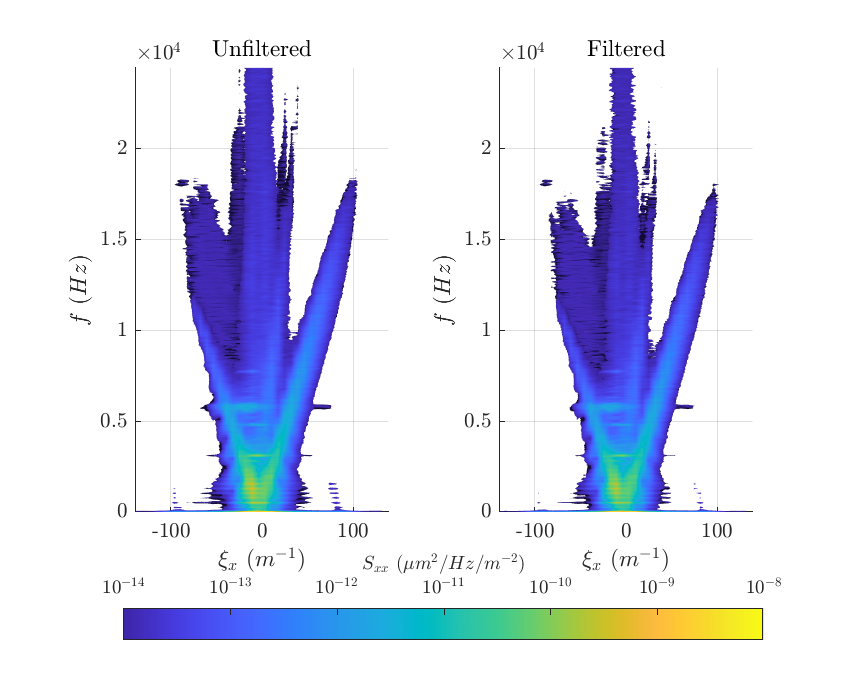
\includegraphics{../matlab/07_multiple_sensor_filtering/lse_spod.eps}
  \caption{A multidimensional power spectrum of an unfiltered wavefront and the same wavefront filtered with the LSE-SPOD method using all 16 additional microphone or accelerometer measurements.  }
  \label{fig:07_lse_spod}
\end{figure}
\begin{figure}
  \centering
  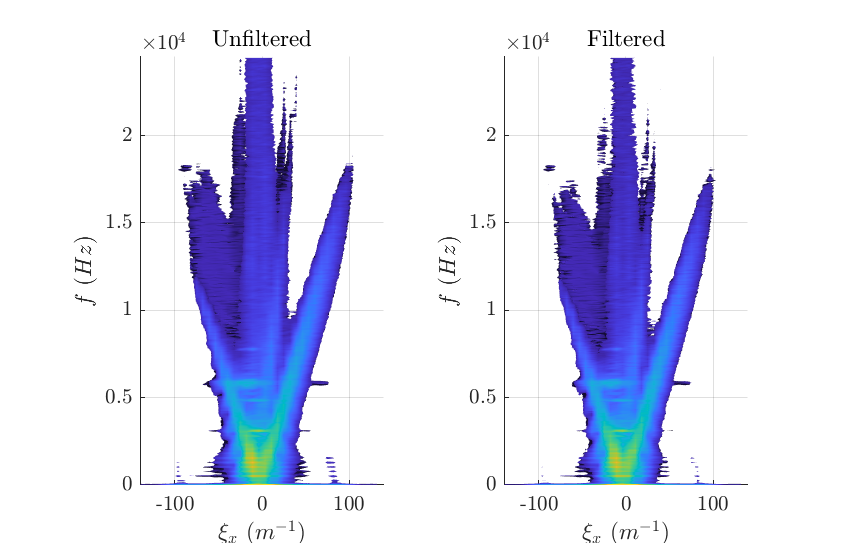
\includegraphics{../matlab/07_multiple_sensor_filtering/lse_mspod.eps}
  \caption{A multidimensional power spectrum of an unfiltered wavefront and the same wavefront filtered with the LSE-MSPOD method using all 16 additional microphone or accelerometer measurements.  }
  \label{fig:07_lse_mspod}
\end{figure}
These plots show the $f$-$\xi_x$ plane of the multidimensional spectrum that captures horizontally-moving (streamwise) plane waves with a portion of the acoustic cone isosurface wrapping behind it.
Both of these methods performed effectively identically to one another with a 14.2\% drop in overall RMS value of the filtered wavefront (both time and space).
There is a significant drop in the signal at the blade-passing frequency and its harmonics, especially at the higher spatial frequencies.
The stationary signal information is also significantly reduced along with the high temporal-frequency acoustic signal.
The aero-optical boundary layer signal is also partially reduced, which is most noticeable at higher temporal-frequencies.
% Some of this lost signal can be restored by increasing the overlap of the temporal frequency blocks, but this also restores some of the unwanted high temporal-frequency contamination.

\begin{table}
  \centering
  \caption{$\opdrms$ ($\mu m$) comparison of using different combinations of additional sensor information in the LSE-MSPOD filtering process.}
  \input{../matlab/07_multiple_sensor_filtering/lse_mspod_table.txt}
  \label{tab:07_lse_mspod_table}
\end{table}

Table \ref{tab:07_lse_mspod_table} shows the time averaged $\opdrms$ of three different data sets at a beam angle through the test-section of $90^\circ$.
The data sets were at Mach numbers of 0.3, 0.4, and 0.5 and had an unfiltered $\opdrms$ of 0.0561, 0.0521, and 0.0824 $\mu m$ respectively.
Note that in the raw processed wavefronts, the $\opdrms$ at a Mach number of 0.3 was higher than the 0.4 case.
There was a significant drop of between 62.6\% and 78.6\% in the $\opdrms$ by removing the Zernike modes corresponding to tip and tilt.
It is at this point the Mach number of 0.4 case has a higher $\opdrms$ than the 0.3 case as would be expected \cite{Gordeyev-2014-jcJndkHM}.
Note that it is standard practice to remove optical tip/tilt from wavefront measurements, since tip/tilt is largely imposed by the measurement optics rather than the actual aero-optical flow.

Table \ref{tab:07_lse_mspod_table} also shows the effect of five different combinations of additional sensors that were used for filtering with the LSE-MSPOD process (the bracketed percentage in Table \ref{tab:07_lse_mspod_table} shows the percent reduction in $\opdrms$ due to the filtering).
The first set was all of the accelerometers which resulted in an additional drop in $\opdrms$ of between 3\% and 5\%.
The second and third sets used either the ambient or duct microphones and those sets had slightly less reduction than the accelerometers.
The fourth set was the test-section sensors comprised of six window mounted accelerometers and four duct mounted microphones.
This set of sensors performed the same as all of the accelerometers, while the use of all of the additional sensors in the last set performed the best, with an additional reduction in $\opdrms$ of 4 to 6\% from the tip/tilt removal cases.

% A velocity filter was also tried in addition to just the tip/tilt removal or in conjunction with tip/tilt and all the sensors being used in the LSE-MSPOD process.
% The velocity filter performed better than the all-sensors removal case by an additional 1.5 to 3\% but some of the narrow-band signals remain.
% When all sensors were used with LSE-MSPOD on the velocity filtered wavefronts an additional 3 to 4\% of the $\opdrms$ was removed compared to just the velocity-filtered case or an additional 8.1\% reduction for only doing tip/tilt removal on the Mach number of 0.3 case or 14.1 and 13.3\% reduction for the 0.4 and 0.5 Mach number cases.

In summary, Table \ref{tab:07_lse_mspod_table} shows that using either the temporal or multidimensional version of the LSE-SPOD filtering technique can help remove some of the narrow-band acoustic and vibration reduction in an optical wavefront.
These temporally narrow-band signals have broadband spatial content that is attenuated.
This additional reduction does seem to be somewhat tied to the number of sensors used with more sensors having a greater impact on the signal reduction.
Since the vibrations and acoustics have the same primary source, the wind-tunnel fan, they seems to do a relatively equivalent job at filtering the optical contamination.
Accelerometers have the benefit of easier installation but the microphones do not necessarily have to be installed inside of the wind-tunnel.
